\documentclass[10pt,A4,]{article}
% \RequirePackage[l2tabu, orthodox]{nag}
\usepackage[a4paper,text={16.5cm,25.2cm},centering,margin=2.6cm]{geometry}
% \usepackage[left=1.0in,top=1.0in,right=1.0in,bottom=1.0in]{geometry}
\newcommand*{\authorfont}{\fontfamily{phv}\selectfont}
\usepackage{hyperref,amsmath,amssymb,bm,url,enumitem,dcolumn,upquote,framed,alltt,textgreek,xfrac,fixltx2e}
\usepackage[australian]{babel}
\usepackage[compact,small]{titlesec}
\setlength{\parskip}{1.2ex}
\setlength{\parindent}{0em}

\def\tightlist{}

\usepackage{ifxetex}
\ifxetex
  \usepackage{fontspec}
  \defaultfontfeatures{Ligatures=TeX} % To support LaTeX quoting style
 \defaultfontfeatures{Ligatures=TeX}
 \setmainfont{Minion Pro}
 \setsansfont[Scale=MatchLowercase]{Myriad Pro}
 \setmonofont[Scale=MatchLowercase]{Ubuntu Mono}
\else
  \usepackage[T1]{fontenc}
  \usepackage[utf8]{inputenc}
  \usepackage{lmodern}
  % \usepackage[full]{textcomp} % directly use the degree (and some other) symbol
\fi

% place after fonts; even better typesetting for improved readability:
% \graphicspath{ {figure/} }
\usepackage{tabularx} % for 'tabularx' environment and 'X' column type
\usepackage{ragged2e}  % for '\RaggedRight' macro (allows hyphenation)
\usepackage{siunitx}
    \sisetup{%
        detect-mode,
        group-digits            = false,
        input-symbols           = ( ) [ ] - + < > *,
        table-align-text-post   = false,
        round-mode              = places,
        round-precision         = 3
        }
% \usepackage[font={small, sf}, labelfont=bf]{caption} % tweaking the captions
\usepackage[font={small}, labelfont=bf]{caption} % tweaking the captions
\usepackage[color=yellow, textsize=tiny]{todonotes}
\frenchspacing%
% \usepackage[kerning=false,protrusion=true,expansion=true]{microtype}

\usepackage{abstract}
\renewcommand{\abstractname}{} % clear the title
\renewcommand{\absnamepos}{empty} % originally center

\renewenvironment{abstract}
{{%
\setlength{\leftmargin}{0mm}
\setlength{\rightmargin}{\leftmargin}%
}%
\relax}
{\endlist}

\makeatletter
\def\@maketitle{%
\newpage
%  \null
%  \vskip 2em%
%  \begin{center}%
\let \footnote \thanks
 {\fontsize{18}{20}\selectfont\raggedright  \setlength{\parindent}{0pt} \@title \par}%
}
%\fi
\makeatother


\setcounter{secnumdepth}{0}





\usepackage{longtable,booktabs}
\setlength\heavyrulewidth{0.1em}
\setlength\lightrulewidth{0.0625em}


\title{Intro R Workshop: Exercise 2  }

\author{\Large \vspace{0.05in} \newline\normalsize\emph{University of the Western Cape}   \and \Large AJ Smit\vspace{0.05in} \newline\normalsize\emph{}  }

\date{}

% PENALTIES
\widowpenalty=1000
\clubpenalty=1000
\doublehyphendemerits=9999 % Almost no consecutive line hyphens
\brokenpenalty=10000 % No broken words across columns/pages
\interfootnotelinepenalty=9999 % Almost never break footnotes

% SECTION, SUBSECETC.TITLES
\usepackage[compact]{titlesec}
\titleformat{\chapter}
  {\normalfont\LARGE\sffamily\bfseries}
  {\thechapter}
  {1em}
  {}
\titleformat{\section}
  {\normalfont\LARGE\sffamily\bfseries}
  {\thesection}
  {1em}
  {}
\titleformat{\subsection}
  {\normalfont\Large\sffamily\bfseries}
  {\thesubsection}
  {1em}
  {}
\titleformat{\subsubsection}
  {\normalfont\large\sffamily\bfseries\slshape}
  {\thesubsubsection}
  {1em}
  {}
% \titlespacing*{<command>}{<left>}{<before-sep>}{<after-sep>}
\titlespacing*{\chapter}
  {0pt}
  {1.2ex plus 1ex minus .2ex}
  {0.5ex plus .1ex minus .1ex}
\titlespacing*{\section}
  {0pt}
  {1.2ex plus 1ex minus .2ex}
  {0.5ex plus .1ex minus .1ex}
\titlespacing*{\subsection}
  {0pt}
  {1.2ex plus 1ex minus .2ex}
  {0.5ex plus .1ex minus .1ex}
\titlespacing*{\subsubsection}
  {0pt}
  {1.2ex plus 1ex minus .2ex}
  {0.5ex plus .1ex minus .1ex}



\newtheorem{hypothesis}{Hypothesis}
\usepackage{setspace}

\makeatletter

\@ifpackageloaded{hyperref}{}{%
\ifxetex
  \usepackage[setpagesize=false, % page size defined by xetex
              unicode=false, % unicode breaks when used with xetex
              xetex]{hyperref}
\else
  \usepackage[colorlinks=true, citecolor=blue, linkcolor=cyan, pdfborder={0 0 0 }, unicode=true]{hyperref} % place after other packages, but before cleveref
\fi
}

\@ifpackageloaded{color}{
    \PassOptionsToPackage{usenames,dvipsnames}{color}
}{%
    \usepackage[usenames,dvipsnames]{color}
}

\usepackage{cleveref} % cleverly cross referencing figures and tables; last package to include
\setcounter{secnumdepth}{2}
\setcounter{tocdepth}{2}

% To use for resetting the numbering of Appendix Tables and Figures:
%\setcounter{table}{0}
%\renewcommand{\thetable}{A\arabic{table}}
%\setcounter{figure}{0}
%\renewcommand{\thefigure}{A\arabic{figure}}

\makeatother
\hypersetup{breaklinks=true,
            bookmarks=true,
            pdfauthor={ (University of the Western Cape) and AJ Smit ()},
             pdfkeywords = {},
            pdftitle={Intro R Workshop: Exercise 2},
            colorlinks=true,
            citecolor=blue,
            urlcolor=blue,
            linkcolor=magenta,
            pdfborder={0 0 0}}
\urlstyle{same}  % don't use monospace font for urls


\begin{document}

% \maketitle

{% \usefont{T1}{pnc}{m}{n}
\setlength{\parindent}{0pt}
\thispagestyle{plain}
{\fontsize{18}{20}\selectfont\raggedright
\maketitle  % title \par
}
{
   \vskip 13.5pt\relax \normalsize\fontsize{11}{12}
\textbf{\authorfont } \hskip 15pt \emph{\small University of the Western Cape}   \par \textbf{\authorfont AJ Smit} \hskip 15pt \emph{\small }   
}
}



\vskip 6.5pt

\noindent 

\section{The
SACTNmonthly\_v4.0.RData}\label{the-sactnmonthly_v4.0.rdata}

Please \emph{exactly} recreate the figure immediately below (you may use
your own colour for the line). Note: in order to calculate a yearly mean
for each of the data points within a year, you will have to use one of
the functions in the \textbf{lubridate} package. There is also the
\texttt{mutate()} function (within the \textbf{dplyr} package) that I
have mentioned before, but which we have not explicitely practiced ---
it will have to be used to receive the result of the \textbf{lubridate}
function that I alluded to above.

\begin{center}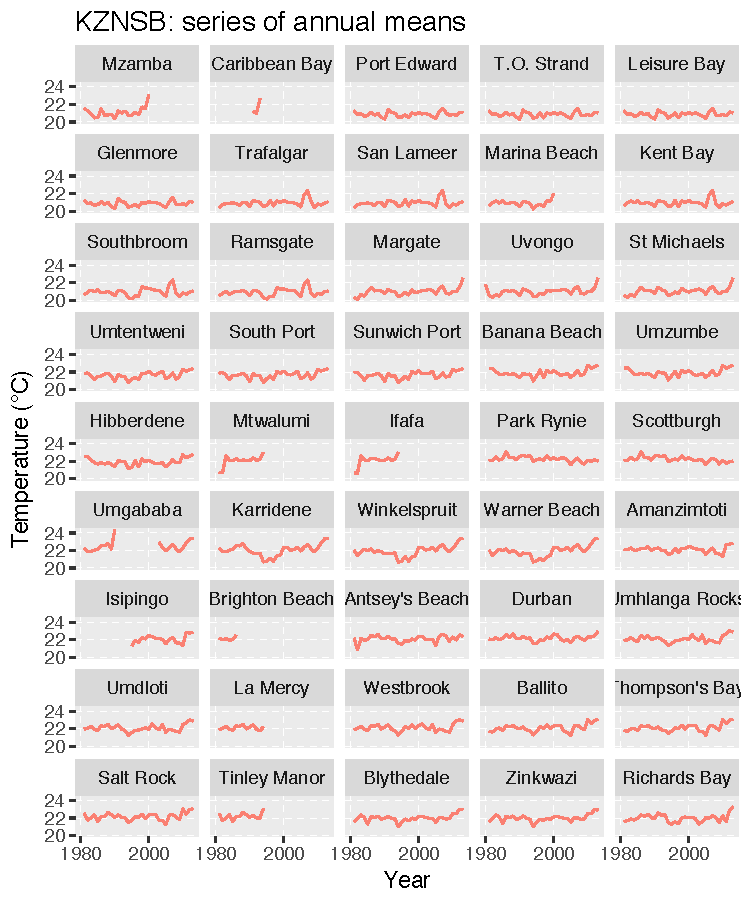
\includegraphics{figures/exercise-1ex-1-1} \end{center}

\section{The data.laminaria.csv data}\label{the-data.laminaria.csv-data}

Please recreate the following figure \emph{exactly} (note: the graph is
not atually meaningful, and it is the incorrect way to display the data;
used here for demonstration purpuses only):

\begin{flushleft}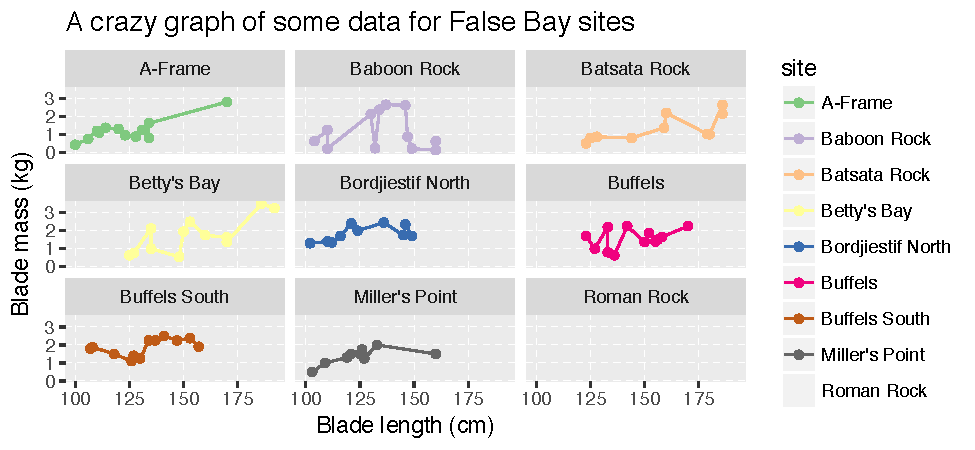
\includegraphics{figures/exercise-1ex-2-1} \end{flushleft}

In the above graph I used one of the palettes included with the Colour
Brewer scale. Unfortunately the plot for Romans Rock is now missing.
Why? Please provide a solution to this problem --- i.e.~make a new graph
where the problem is no longer present. Combine the graphs as two
sub-plots (i.e.~a figure labeled `A' and `B') using the facility offered
by the \texttt{ggpubr} package.

\section{The ToothGrowth data}\label{the-toothgrowth-data}

These data reside in \texttt{datasets::ToothGrowth}. Please produce a
graph like the one below. The adjustment of the error bars (here showing
±SD) is a bit tricky, so you will have to figure out how to consult the
help files, or find alternative help somewhere using an internet search.

\begin{center}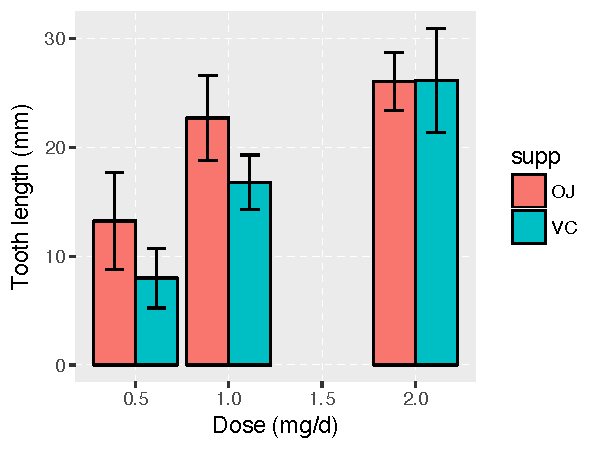
\includegraphics{figures/exercise-1ex-3-1} \end{center}

\end{document}
